\chapter{Sicurezza}
\section{Privacy e sicurezza}
L'adozione delle tecnologie basate sulla blockchain, si è progressivamente ampliata oltre il settore delle criptovalute, trovando applicazione in ambiti come quello della protezione della privacy \cite{borroni_blockchain_2019}.
La spinta verso la decentralizzazione deriva principalmente dalle crescenti preoccupazioni degli utenti riguardo alla perdita di controllo sui propri dati personali archiviati online \cite{rodota_quattro_paradigmi_2018} \cite{alpa_identita_digitale_2017}.
A tal riguardo, la struttura stessa della blockchain offre potenzialità per tutelare la riservatezza delle informazioni personali; tuttavia, l'analisi dei metadati può renderla vulnerabile in determinati contesti. Di conseguenza, senza un'adeguata progettazione,
«\textit{decentralized infrastructures intended to promote individual privacy and autonomy might turn out to be much more vulnerable to governmental or corporate surveillance than their centralized counterparts}» \cite{de_filippi_interplay_2016}.
In questa prospettiva, non va dimenticato che la natura pseudonima di molte
reti che si basano sulla blockchain consente agli individui la possibilità di
condurre le proprie transazioni su base peer-to-peer, senza la necessità di
rivelare la propria identità alle controparti.
\subsection{Il difficile rapporto tra trasparenza e privacy}
Allo stesso tempo, la trasparenza derivante dalle distributed ledger technologies è tale che chiunque ha la possibilità di accedere alla
cronologia di tutte le transazioni memorizzate sulla blockchain, affidandosi così all’analisi dei dati in essa contenuti per ricavare informazioni potenzialmente sensibili \cite{marr_history_blockchain_2018}.
Se il sistema non viene progettato con la dovuta attenzione, la trasparenza potrebbe compromettere la tutela della privacy degli utenti, in quanto questi avrebbero
accesso ai dati di tutti gli altri utenti presenti sulla piattaforma e quindi si avrebbe un miglioramento della trasparenza 
a discapito però della privacy.\\
Pertanto, in assenza di soluzioni tecniche adeguate per salvaguardare la riservatezza delle comunicazioni online, le infrastrutture decentralizzate, pensate per favorire privacy e autonomia, 
rischiano di risultare più esposte al controllo di governi o aziende rispetto ai sistemi centralizzati.
Resta comunque una notevole incertezza riguardo alla capacità di soluzioni alternative e decentralizzate di affrontare efficacemente le problematiche legate alla protezione dei dati.
Nonostante ciò, i sistemi decentralizzati, come la blockchain, hanno suscitato un crescente interesse nella comunità accademica, che sta approfondendo il potenziale utilizzo delle DLTs in ambito privacy.
\\Per comprendere meglio le questioni legate alla protezione dei dati personali, è fondamentale esaminare due aspetti principali:
\begin{itemize}
    \item l'individuazione del soggetto responsabile della definizione delle modalità di trattamento dei dati personali
    \item l'identificazione di chi controlla la conservazione e gestione dei dati
\end{itemize}
La natura decentralizzata della blockchain non solo garantisce livelli più elevati di protezione dei dati personali, ma conferisce agli utenti un maggiore controllo sulle proprie informazioni, permettendo loro di gestirle autonomamente durante gli scambi. Questa tecnologia è stata infatti descritta dalla dottrina come un vero e proprio «\textit{sistema di cloud computing decentralizzato}».
\\In tale contesto, il principale vantaggio offerto dai sistemi decentralizzati risiede nella possibilità per gli utenti di assumere un controllo diretto sulla gestione dei propri dati, inoltre, le informazioni generate, condivise e raccolte dagli utenti stessi potrebbero essere messe a disposizione o vendute per fini comuni,
consentendo l'accesso anche a terze parti. Questo approccio ricorda quello degli open data, ma con meccanismi e logiche significativamente diversi.
\\Per quanto riguarda la struttura, gran parte delle architetture decentralizzate disponibili per gli utenti sono progettate con l'obiettivo di favorire la privacy, focalizzandosi su almeno uno dei due paradigmi fondamentali: la riservatezza dei dati e la “sovranità” su di essi.
\\In questa prospettiva, la decentralizzazione che caratterizza la blockchain offre un potenziale significativo per ridurre le asimmetrie informative che si verificano quando una delle parti coinvolte in una transazione possiede informazioni rilevanti che l'altra parte non conosce, le quali, nei sistemi centralizzati, tendono a creare vantaggi per gli operatori a discapito degli utenti.
\\Tuttavia, va evidenziato che, allo stato attuale, persistono numerose complessità nel comprendere appieno come privacy e trasparenza possano interagire tra loro.
In una società “trasparente”, da un lato, qualsiasi parte interessata può facilmente accedere alle informazioni. Questo implica che la trasparenza sociale possa compromettere il diritto alla privacy. Di conseguenza, è legittimo associare una crescente trasparenza delle informazioni a un ridotto rispetto del diritto alla privacy.
In tale contesto, la trasparenza offerta dalle DLTs non è né totale né incondizionata. 
\subsection{Blockchain Permissioned e Permissionless}
Le diverse tipologie di blockchain, infatti, possono garantire vari livelli di trasparenza. Esistono, in particolare, due tipologie di blockchain: 
\begin{itemize}
    \item [\textit{permissioned}:] in cui una sola autorità ha il permesso di scrivere sulla blockchain e detiene praticamente il controllo del sistema distribuito.
    \item [\textit{permissionless}:] in cui chiunque può partecipare come nodo, verificare transazioni e aggiungere blocchi al registro e tutti i dati delle transazioni sono visibili e accessibili a chiunque abbia accesso alla rete, anche se non tutti possono necessariamente scrivere nella blockchain (ma chiunque può leggere i dati).
\end{itemize}
Soprattutto nel caso delle blockchain permissioned, le transazioni (o scambi, scrittura delle informazioni) avvengono all’interno di un ecosistema chiuso, dove i dati registrati sono mantenuti riservati e le identità dei partecipanti sono note.
\subsection{Crittografia End-to-End e responsabilità degli algoritmi}
Da un punto di vista pratico, i problemi di privacy legati al livello di trasparenza della blockchain possono essere attenuati mediante la crittografia “end-to-end” delle comunicazioni, che utilizza chiavi private e pubbliche, anziché una chiave unica per crittografare e decrittografare.
\\Il principio implica che, ove possibile, le operazioni del protocollo di comunicazione debbano essere eseguite ai punti finali di un sistema di comunicazione, o comunque il più vicino possibile alla risorsa da controllare.
In particolare, le aspettative sociali riguardo la trasparenza e la supervisione degli algoritmi sono in forte crescita, con l’obiettivo di rendere i sistemi decisionali automatizzati più responsabili, trasparenti e governabili. Si sta cercando di dotare questi sistemi di nuovi strumenti tecnologici per verificare che le decisioni automatizzate rispettino standard di equità giuridica. 
Garantire la responsabilità attraverso valutazioni d’impatto degli algoritmi (AIA), audit e certificazioni dovrebbe diventare parte integrante delle iniziative politiche e legali in questo ambito, considerando che la blockchain, al momento, non è stata ancora completamente implementata.
\\
\\
\\
\section{Web 3.0}
L'idea del Web 3.0 è stata inzialmente utilizzata in stretta connessione con il concetto di web semantico, terminologia creata da Berners Lee in un articolo di \textit{Scientific American} del 2001 per descrivere un nuovo web. 
La sua idea è che, così come il web 2.0 permette di collegare pagine web, a livello di visualizzazione, il web semantico deve permettere non solo di collegare pagine tra loro ma anche i dati contenuti in esse \cite{ted_youtube}.
La visone del web semantico è una visione di dati interconnessi e navigabili che possono essere usati da chiunque. L'esigenza di socializzazione dei dati è ancora più importante oggi che l'intelligenza artificiale può costruire modelli a partire dai dati grezzi, sulla base di algoritmi generali.
L'obiettivo del web 3.0, riconosciuto da Gavin Wood, co fondatore di Ethereum, è quello di creare un web decentralizzato, dove i dati sono posseduti dagli utenti e non da poche aziende. Sta nascendo la consapevolezza di re-decentralizzare i servizi web.
Questa idea è diffusa da molto tempo, ma adesso finalmente esistono le tencologie che permettono di realizzarla, come la blockchain.
Così si potrebbero ottenere numerosi vantaggi, tra i quali:
\begin{itemize}
    \item [\textit{Decentralizzazione}:] Non è necessario alcun permesso da parte di un'autorità centrale per caricare qualcosa sul web. Questo fornisce una protezione contro qualsiasi forma di censura e controllo. Il web tornerebbe ad essere un sistema neutrale.
    \item [\textit{Democratizzazione}:] E' possibile offrire un accesso a chiunque abbia una connessione a internet, senza discriminazioni su età, sesso, razza, religione e posizione geografica.
    \item [\textit{Uptime dei servizi}:] Non essendoci nodi centrali, non esiste un punto di fallimento. Se un nodo va giù, il servizio è comunque disponibile.
    \item [\textit{Possesso dei dati}:] Gli utenti riprenderebbero possesso dei propri dati potendo decidere con chi condividerli e in che modo, potendo potenzialmente guadagnare dalla vendita dei propri dati attraverso smart contracts alle grandi multinazionali come FaceBook e Google le quali hanno tantissime informazioni sugli utenti e gli advertiser che pubblicano le pubblicità sulle loro piattaforme pagano milioni per avere questi dati.
    \item [\textit{Persistenza dei dati}:] I dati non possono essere cancellati, a meno che non venga cancellata l'intera blockchain, in quanto verranno salvati in maniera ridondante su diversi nodi distribuiti indipendentemente.
\end{itemize}
\begin{figure}[h]
    \caption{Livelli del web 3.0}
    \centering
    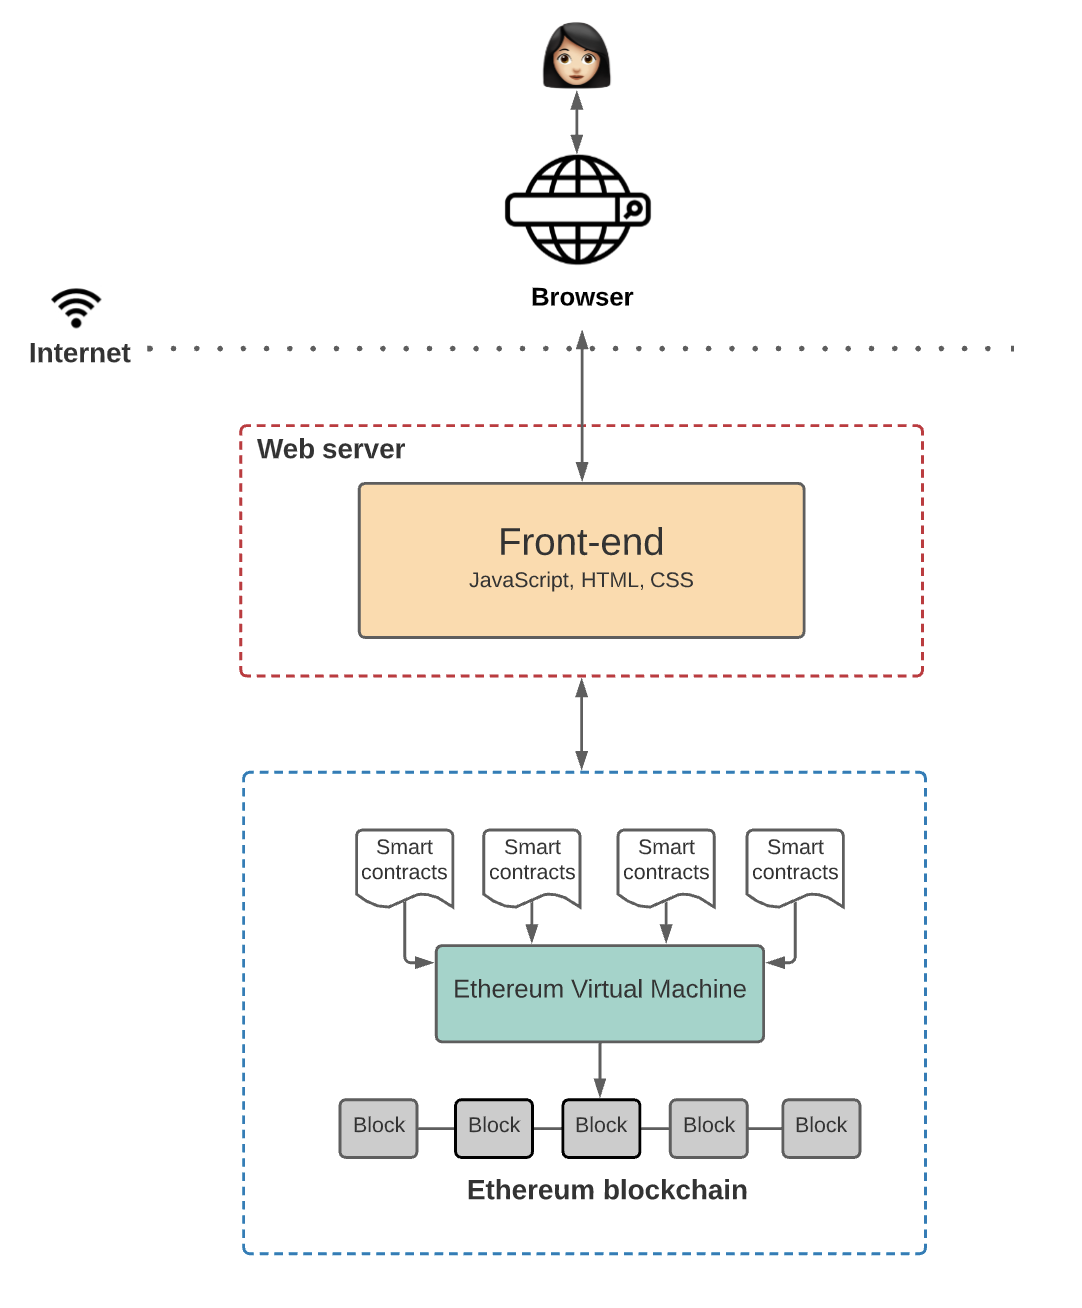
\includegraphics[width=0.65\textwidth]{Immagini/web_30.png}
\end{figure}
L'architettura del web 3.0 non è ancora stata definita in maniera chiara e ufficiale, ma la sua caratteristica chiave sarà certamente l'assenza
di divisione netta tra utenti e fornitori di servizi. Per esempio quando ci colleghiamo a FaceBook siamo utenti e FaceBook agisce come provider 
offrendoci un servizio in cambio dei nostri dati personali. La prossima iterazione del web permetterà di eliminare questa contrapposizione netta, perchè
gli utenti potranno essere anche fornitori di servizi, almeno nelle Blockchain pubbliche.
